\documentclass[aspectratio=169,11pt]{beamer}

\usetheme{SimplePlus}

\usepackage{amsmath}
\usepackage{amssymb}
\usepackage{booktabs}
\usepackage{graphicx}
\usepackage{array}

\graphicspath{{images/lecture-3/}}

\title{S181M116 Derivatives and Alternative Investments}
\subtitle{Lecture 3: Interest Rates, Bonds, Swaps, and Fixed-Income Inputs}
\author{Swapnil Singh}
\institute{Lietuvos Bankas and Kaunas University of Technology}
\date{}

\newcommand{\PV}{\mathrm{PV}}
\newcommand{\FV}{\mathrm{FV}}
\newcommand{\DF}{\mathrm{DF}}
\newcommand{\bp}{\mathrm{bp}}
\newcommand{\notional}{N}
\newcommand{\FRA}{\mathrm{FRA}}
\newcommand{\SOFR}{\mathrm{SOFR}}
\newcommand{\CF}{\mathrm{CF}}
\newcommand{\CTD}{\mathrm{CTD}}
\newcommand{\Dur}{D}
\newcommand{\Conv}{C}

\AtBeginSection[]{
    \begin{frame}[plain,noframenumbering]
        \vfill
        \begin{center}
            {\usebeamerfont{subtitle}\usebeamercolor[fg]{structure}Section \thesection\par}
            \vspace{0.5em}
            {\usebeamerfont{title}\usebeamercolor[fg]{titlelike}\insertsectionhead\par}
        \end{center}

        \vspace{1.2em}
        \begin{center}
            \begin{minipage}{0.72\textwidth}
                \tableofcontents[currentsection,hideothersubsections]
            \end{minipage}
        \end{center}
        \vfill
    \end{frame}
}

\begin{document}

\begin{frame}
    \titlepage
\end{frame}

\begin{frame}{Today}
    \begin{enumerate}
        \item Why derivative pricing needs a discount curve, not one rate.
        \item How compounding conventions, zero rates, and discount factors fit together.
        \item How to price bonds and bootstrap a simple zero curve.
        \item How forward rates and FRAs use the same curve logic.
        \item How duration and convexity measure interest-rate exposure.
        \item How Treasury bond futures and SOFR futures are quoted and hedged.
        \item How swaps are structured, priced, and valued after rates move.
    \end{enumerate}
\end{frame}

\begin{frame}{Core Message}
    \begin{block}{Fixed-income derivative pricing has three questions}
        \begin{enumerate}
            \item \textbf{Cash-flow dates:} when is each payment made?
            \item \textbf{Discounting inputs:} which discount factor applies to each date?
            \item \textbf{Rate sensitivity:} how does value change when the curve moves?
        \end{enumerate}
    \end{block}

    \vspace{0.5em}
    The ``risk-free rate'' in a formula is a shorthand.
    Market implementation uses a term structure of discount factors, plus conventions.
\end{frame}

\section{Interest Rate Inputs}

\begin{frame}{Many Rates, One Pricing Problem}
    \begin{columns}[T]
        \begin{column}{0.48\textwidth}
            \begin{block}{Rates differ by}
                \begin{itemize}
                    \item maturity;
                    \item collateral;
                    \item credit risk;
                    \item liquidity;
                    \item tax and regulation;
                    \item compounding and day count.
                \end{itemize}
            \end{block}
        \end{column}
        \begin{column}{0.48\textwidth}
            \begin{block}{Basis point}
                \[
                    1\bp=0.01\%=0.0001.
                \]
                A move from 4.25\% to 4.40\% is 15 basis points.
            \end{block}

            \begin{alertblock}{Practical lesson}
                Quoting a rate is not enough. We must also know the convention behind it.
            \end{alertblock}
        \end{column}
    \end{columns}
\end{frame}

\begin{frame}{Reference Rates}
    \begin{columns}[T]
        \begin{column}{0.50\textwidth}
            \begin{block}{Old benchmark logic}
                LIBOR was intended to measure unsecured term bank borrowing.
                The rate was usually known at the start of the interest period.
            \end{block}
        \end{column}
        \begin{column}{0.46\textwidth}
            \begin{block}{New benchmark logic}
                Overnight risk-free rates such as SOFR are based on overnight transactions.
                Period rates are often compounded from daily observations.
            \end{block}
        \end{column}
    \end{columns}

    \vspace{0.6em}
    \begin{alertblock}{Derivative pricing implication}
        The relevant curve depends on currency, collateral, payment timing, and contract terms.
        A Treasury curve and an overnight-indexed swap discount curve need not agree.
    \end{alertblock}
\end{frame}

\begin{frame}{Discrete Compounding}
    If amount \(A\) is invested for \(n\) years at annual rate \(R\), compounded \(m\) times per year:
    \[
        \FV=A\left(1+\frac{R}{m}\right)^{mn}.
    \]

    \begin{exampleblock}{Same quote, different compounding}
        A rate of 10\% for one year gives
        \[
            100(1.10)=110.00
        \]
        with annual compounding, but
        \[
            100\left(1+\frac{0.10}{2}\right)^2=110.25
        \]
        with semiannual compounding.
    \end{exampleblock}
\end{frame}

\begin{frame}{Continuous Compounding}
    As compounding becomes arbitrarily frequent:
    \[
        \FV=Ae^{Rn},
        \qquad
        \PV=\FV e^{-Rn}.
    \]

    \begin{block}{Conversion}
        If \(R_m\) is compounded \(m\) times per year and \(R_c\) is the equivalent continuously compounded rate,
        \[
            R_c=m\ln\left(1+\frac{R_m}{m}\right),
            \qquad
            R_m=m\left(e^{R_c/m}-1\right).
        \]
    \end{block}

    \begin{exampleblock}{Semiannual to continuous}
        \(6\%\) with semiannual compounding is
        \(2\ln(1.03)\approx 5.91\%\) with continuous compounding.
    \end{exampleblock}
\end{frame}

\begin{frame}{Discount Factors}
    \begin{columns}[T]
        \begin{column}{0.52\textwidth}
            \begin{block}{Core object}
                The discount factor \(P(0,T)\) is the price today of receiving one unit of currency at time \(T\).
            \end{block}

            If \(R(0,T)\) is a continuously compounded zero rate,
            \[
                P(0,T)=e^{-R(0,T)T}.
            \]
            \[
                R(0,T)=-\frac{1}{T}\ln P(0,T).
            \]

            Derivatives discount each dated cash flow with the discount factor for that date.
        \end{column}
        \begin{column}{0.44\textwidth}
            \begin{center}
                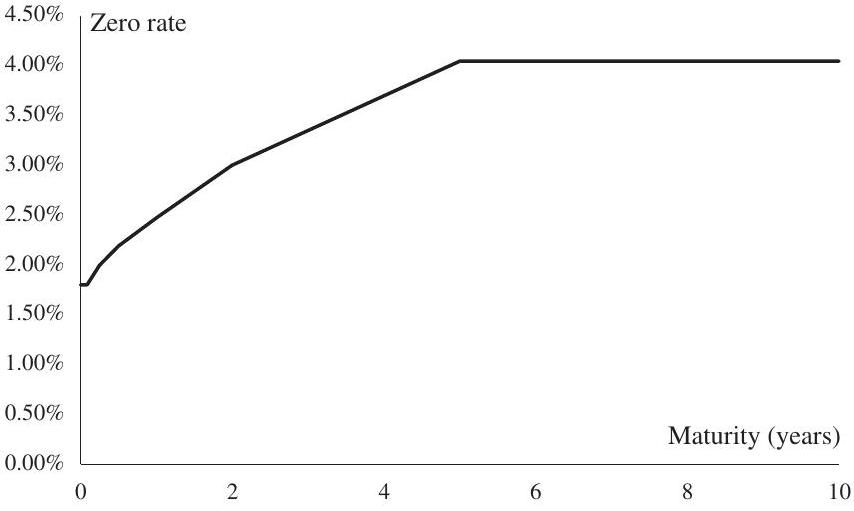
\includegraphics[width=\linewidth,height=0.62\textheight,keepaspectratio]{b71beec3-7c42-4186-a630-199cabe63c35-176_511_854_1798_457.jpg}
            \end{center}
        \end{column}
    \end{columns}
\end{frame}

\section{Zero Curves and Bonds}

\begin{frame}{Zero Rates}
    \begin{block}{Definition}
        The \(T\)-year zero rate is the rate that prices a zero-coupon payoff at \(T\):
        \[
            P(0,T)=e^{-R(0,T)T}.
        \]
    \end{block}

    \begin{itemize}
        \item A zero-coupon bond pays once, at maturity.
        \item A zero curve gives zero rates or discount factors for many maturities.
        \item A single yield is a summary statistic; a curve is an input to valuation.
    \end{itemize}

    \begin{alertblock}{Why this matters}
        A coupon bond or swap has cash flows on several dates, so each cash flow needs its own discount factor.
    \end{alertblock}
\end{frame}

\begin{frame}{Bond Pricing from the Zero Curve}
    A coupon bond is a package of dated cash flows.
    If cash flow \(C_i\) is paid at date \(t_i\), its value is
    \[
        B=\sum_i C_i P(0,t_i).
    \]

    With continuously compounded zero rates:
    \[
        B=\sum_i C_i e^{-R(0,t_i)t_i}.
    \]

    \begin{block}{Yield to maturity}
        The yield \(y\) is the single rate that solves
        \[
            B=\sum_i C_i e^{-y t_i}.
        \]
        It prices the bond, but it hides the shape of the term structure.
    \end{block}
\end{frame}

\begin{frame}{Bond Price Example}
    A bond pays 4 in one year and 104 in two years.
    The one-year zero rate is 3\% and the two-year zero rate is 3.8\%, both continuously compounded.

    \[
        B=4e^{-0.03(1)}+104e^{-0.038(2)}.
    \]

    \[
        B\approx 3.88+96.38=100.26.
    \]

    \begin{alertblock}{Common mistake}
        Do not discount both cash flows with the two-year yield just because the bond matures in two years.
        The first coupon is a one-year cash flow.
    \end{alertblock}
\end{frame}

\begin{frame}{Bootstrapping a Zero Curve}
    \begin{block}{Recursive logic}
        \begin{enumerate}
            \item Start with the shortest maturity instrument.
            \item Infer the first discount factor.
            \item Move to the next maturity.
            \item Subtract the value of earlier cash flows using known discount factors.
            \item Solve for the new discount factor.
        \end{enumerate}
    \end{block}

    \begin{exampleblock}{One-year step}
        A six-month zero costs 98 per 100, so \(P(0,0.5)=0.98\).
        A one-year bond costs 101 and pays 3 in six months and 103 in one year:
        \[
            101=3(0.98)+103P(0,1),
            \qquad
            P(0,1)=0.9511.
        \]
    \end{exampleblock}
\end{frame}

\begin{frame}{Forward Rates from Zero Rates}
    A forward rate is a rate agreed today for a future period.
    With continuous compounding:
    \[
        e^{R(0,T_2)T_2}
        =
        e^{R(0,T_1)T_1}e^{F(T_1,T_2)(T_2-T_1)}.
    \]

    Therefore
    \[
        F(T_1,T_2)=
        \frac{R(0,T_2)T_2-R(0,T_1)T_1}{T_2-T_1}.
    \]

    In discount-factor form:
    \[
        e^{-F(T_1,T_2)(T_2-T_1)}
        =
        \frac{P(0,T_2)}{P(0,T_1)}.
    \]
\end{frame}

\begin{frame}{Forward Rate Example}
    The one-year zero rate is 3\% and the two-year zero rate is 4\%, both continuously compounded.

    \[
        F(1,2)=\frac{0.04(2)-0.03(1)}{2-1}=0.05.
    \]

    The forward rate for year 2 is 5\%.

    \begin{block}{Interpretation}
        Forward rates are break-even rates implied by the current zero curve.
        They are pricing rates, not necessarily unbiased forecasts of future spot rates.
    \end{block}

    \begin{itemize}
        \item Risk premia, convexity, liquidity, and segmentation can all matter.
        \item For derivative pricing, internal consistency with current prices is the key point.
    \end{itemize}
\end{frame}

\section{FRAs and Rate Risk}

\begin{frame}{Forward Rate Agreements}
    \begin{block}{Definition}
        An FRA locks in an interest rate for a future borrowing or lending period.
        The notional is used to calculate interest, but the notional is not exchanged.
    \end{block}

    Let:
    \begin{itemize}
        \item \(\notional\) be notional principal;
        \item \(K\) be the contract rate;
        \item \(R\) be the market reference rate observed at reset;
        \item \(\tau\) be the accrual fraction.
    \end{itemize}

    For a receive-floating, pay-fixed FRA, the reset-date payoff is commonly written as
    \[
        \frac{\notional \tau (R-K)}{1+R\tau}.
    \]
\end{frame}

\begin{frame}{FRA Settlement Example}
    \small
    A trader receives floating and pays fixed on an FRA with:
    \[
        \notional=20{,}000{,}000,\qquad
        K=4.00\%,\qquad
        R=4.60\%,\qquad
        \tau=0.25.
    \]

    \[
        \frac{20{,}000{,}000(0.25)(0.046-0.040)}
        {1+0.046(0.25)}
        \approx 29{,}659.
    \]

    \begin{block}{Why positive?}
        The trader locked in paying 4.00\%, and the market rate moved to 4.60\%.
        The payoff compensates for the interest-rate difference, discounted back to the reset date.
    \end{block}
\end{frame}

\begin{frame}{Duration}
    If a bond price is
    \[
        B=\sum_i C_i e^{-y t_i},
    \]
    its Macaulay duration is
    \[
        \Dur=\frac{\sum_i t_i C_i e^{-y t_i}}{B}.
    \]

    Differentiating the bond price gives the first-order approximation
    \[
        \frac{\Delta B}{B}\approx -\Dur\Delta y.
    \]

    \begin{itemize}
        \item Duration is a weighted-average cash-flow date.
        \item Longer-duration bonds are more sensitive to yield changes.
        \item If yields rise, bond values fall; if yields fall, bond values rise.
    \end{itemize}
\end{frame}

\begin{frame}{Duration Example}
    \small
    A bond pays 5 in one year and 105 in two years.
    The continuously compounded yield is 4\%.

    \[
        B=5e^{-0.04}+105e^{-0.08}\approx 101.78.
    \]

    \[
        \Dur=
        \frac{1(5e^{-0.04})+2(105e^{-0.08})}{101.78}
        \approx 1.95.
    \]

    For a 20 basis point yield increase:
    \[
        \frac{\Delta B}{B}\approx -1.95(0.002)=-0.0039.
    \]

    The duration approximation predicts a price decline of about 0.39\%.
\end{frame}

\begin{frame}{Convexity}
    \begin{columns}[T]
        \begin{column}{0.52\textwidth}
            Duration is a linear approximation, but bond prices are curved functions of yields.

            \[
                \Conv=\frac{\sum_i t_i^2 C_i e^{-y t_i}}{B}.
            \]

            \[
                \frac{\Delta B}{B}
                \approx
                -\Dur\Delta y+\frac{1}{2}\Conv(\Delta y)^2.
            \]

            \begin{alertblock}{Intuition}
                Convexity improves the approximation when yield changes are large.
            \end{alertblock}
        \end{column}
        \begin{column}{0.44\textwidth}
            \begin{center}
                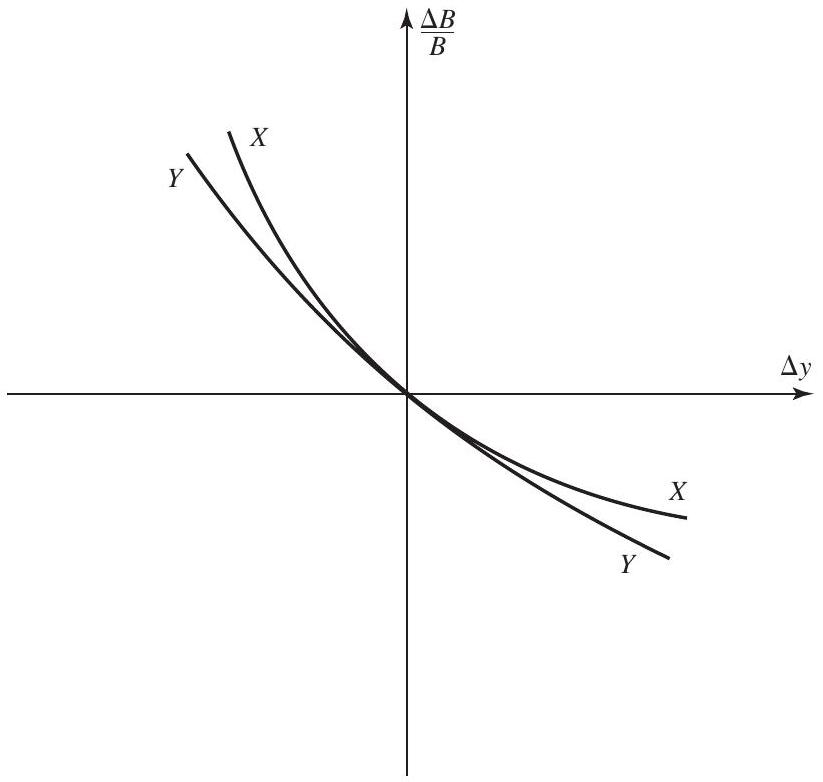
\includegraphics[width=\linewidth,height=0.62\textheight,keepaspectratio]{b71beec3-7c42-4186-a630-199cabe63c35-116_782_823_1490_455.jpg}
            \end{center}
        \end{column}
    \end{columns}
\end{frame}

\begin{frame}{Adding Convexity}
    Suppose a bond has duration 6.8 and convexity 55.
    Yields increase by 50 basis points, so \(\Delta y=0.005\).

    \[
        \text{Duration effect}=-6.8(0.005)=-3.40\%.
    \]

    \[
        \text{Convexity correction}
        =
        \frac{1}{2}(55)(0.005)^2
        =
        0.06875\%.
    \]

    \[
        \frac{\Delta B}{B}
        \approx
        -3.40\%+0.06875\%
        =
        -3.33125\%.
    \]
\end{frame}

\section{Interest Rate Futures}

\begin{frame}{Fixed-Income Conventions}
    Fixed-income markets are convention-heavy.

    \begin{columns}[T]
        \begin{column}{0.48\textwidth}
            \begin{block}{Day count}
                Interest accrual depends on the rule used to convert calendar days into year fractions:
                actual/actual, actual/360, 30/360, and others.
            \end{block}
        \end{column}
        \begin{column}{0.48\textwidth}
            \begin{block}{Clean versus dirty price}
                Treasury bonds are usually quoted as clean prices.
                The actual settlement amount is
                \[
                    \text{dirty price}=\text{clean price}+\text{accrued interest}.
                \]
            \end{block}
        \end{column}
    \end{columns}

    \begin{alertblock}{Implementation lesson}
        Classroom examples often use exact year fractions. Market pricing must handle settlement dates, accrued interest, holidays, and interpolation.
    \end{alertblock}
\end{frame}

\begin{frame}{Treasury Bond Futures}
    \begin{block}{Delivery option}
        The short futures position chooses from a basket of deliverable Treasury bonds.
        Because the bonds differ, the exchange uses conversion factors.
    \end{block}

    \begin{block}{Conversion factor}
        Ignoring accrued interest, the invoice price is approximately
        \[
            \text{futures settlement price}\times \CF.
        \]
    \end{block}

    The full invoice amount is
    \[
        \text{invoice amount}
        =
        \text{futures settlement price}\times \CF
        +\text{accrued interest}.
    \]
\end{frame}

\begin{frame}{Cheapest-to-Deliver}
    \small
    The short chooses the bond that is cheapest to deliver.
    Ignoring accrued interest and delivery timing:
    \[
        \text{delivery cost}
        =
        \text{cash bond price}-(\text{futures price})\times \CF.
    \]

    \begin{center}
        \begin{tabular}{@{}lccc@{}}
            \toprule
            Bond & Cash price & \(\CF\) & Cost if futures price is 112 \\
            \midrule
            A & 118.20 & 1.0500 & \(118.20-112(1.0500)=0.60\) \\
            B & 124.40 & 1.1030 & \(124.40-112(1.1030)=0.864\) \\
            C & 110.10 & 0.9800 & \(110.10-112(0.9800)=0.34\) \\
            \bottomrule
        \end{tabular}
    \end{center}

    \begin{exampleblock}{Result}
        Bond C is cheapest to deliver because it has the lowest delivery cost.
    \end{exampleblock}
\end{frame}

\begin{frame}{Futures Price from a Known CTD Bond}
    If the cheapest-to-deliver bond is known and delivery options are ignored:
    \[
        F_0\approx \frac{(B_0-I)e^{rT}}{\CF}.
    \]

    \begin{description}
        \item[\(B_0\)] current dirty price of the CTD bond;
        \item[\(I\)] present value of coupons received before delivery;
        \item[\(r\)] financing rate;
        \item[\(T\)] time to delivery;
        \item[\(\CF\)] conversion factor.
    \end{description}

    \begin{block}{Connection to Lecture 2}
        This is cash-and-carry logic with coupons, accrued interest, conversion factors, and delivery options added.
    \end{block}
\end{frame}

\begin{frame}{SOFR Futures}
    Short-term interest-rate futures settle on reference rates.
    Older contracts were linked to LIBOR; the post-LIBOR U.S. market uses SOFR futures.

    \[
        \text{futures quote}=100-\text{annualized rate}.
    \]

    \begin{exampleblock}{Quote interpretation}
        A SOFR futures quote of 96.80 implies
        \[
            100-96.80=3.20\%.
        \]
        If the quote falls to 96.65, the implied rate rises to 3.35\%.
    \end{exampleblock}

    \begin{alertblock}{Direction}
        Falling interest-rate futures prices mean rising implied rates.
    \end{alertblock}
\end{frame}

\begin{frame}{Compounding and Convexity in Rate Futures}
    \small
    SOFR for a longer period is built from overnight rates compounded over the period:
    \[
        \left[\prod_{i=1}^n \left(1+r_i\frac{d_i}{360}\right)-1\right]
        \frac{360}{D}.
    \]

    \begin{itemize}
        \item \(r_i\) is the annualized overnight rate for day \(i\).
        \item \(d_i\) is the number of calendar days covered by that rate.
        \item \(D=\sum_i d_i\).
    \end{itemize}

    \begin{block}{Futures versus forwards}
        Futures rates and forward rates can differ because futures settle daily.
        Daily settlement creates a convexity effect when futures payoffs are correlated with rates.
    \end{block}
\end{frame}

\begin{frame}{Duration-Based Futures Hedging}
    A bond portfolio loses value when yields rise.
    A manager can short interest-rate futures so that rate increases create futures gains.

    \[
        N^*=\frac{P D_P}{F D_F}.
    \]

    If portfolio yields and futures-implied yields do not move one-for-one:
    \[
        N^*=\frac{P D_P}{F D_F}
        \frac{\Delta y_P}{\Delta y_F}.
    \]

    \begin{description}
        \item[\(P\)] portfolio value;
        \item[\(D_P\)] portfolio duration;
        \item[\(F\)] futures contract price;
        \item[\(D_F\)] duration of the futures deliverable exposure.
    \end{description}
\end{frame}

\begin{frame}{Duration Hedge Example}
    A bond portfolio is worth EUR 40 million and has duration 5.5.
    The futures contract price is EUR 120,000 and the deliverable exposure duration is 7.2.

    \[
        N^*=
        \frac{40{,}000{,}000(5.5)}
        {120{,}000(7.2)}
        \approx 254.6.
    \]

    The manager shorts about 255 futures contracts.

    \begin{alertblock}{Residual risks}
        The hedge can fail when the yield curve twists, credit spreads move, duration changes, convexity matters, or the cheapest-to-deliver bond changes.
    \end{alertblock}
\end{frame}

\section{Interest Rate Swaps}

\begin{frame}{Plain Vanilla Interest Rate Swap}
    \begin{columns}[T]
        \begin{column}{0.52\textwidth}
            \begin{block}{Mechanics}
                A fixed-for-floating swap exchanges fixed interest payments for floating interest payments on a notional principal.
            \end{block}

            \begin{itemize}
                \item One party pays fixed rate \(S\).
                \item The other pays a floating reference rate.
                \item The notional calculates interest but is not exchanged.
                \item Payments are netted on each payment date.
            \end{itemize}
        \end{column}
        \begin{column}{0.44\textwidth}
            \begin{center}
                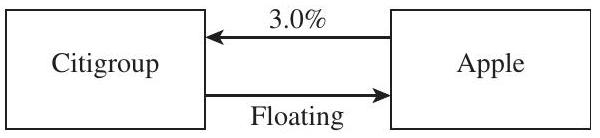
\includegraphics[width=\linewidth,height=0.62\textheight,keepaspectratio]{b71beec3-7c42-4186-a630-199cabe63c35-174_138_600_339_457.jpg}
            \end{center}
        \end{column}
    \end{columns}
\end{frame}

\begin{frame}{Swap Net Payments}
    Suppose payments occur every \(\tau\) years.
    If the fixed rate is \(S\) and the floating rate set for the period is \(L\), the net payment from the fixed payer to the floating payer is
    \[
        \notional\tau(S-L).
    \]

    \begin{columns}[T]
        \begin{column}{0.48\textwidth}
            \begin{block}{If \(S>L\)}
                The fixed payer pays the difference.
            \end{block}
        \end{column}
        \begin{column}{0.48\textwidth}
            \begin{block}{If \(L>S\)}
                The fixed payer receives the difference.
            \end{block}
        \end{column}
    \end{columns}

    \vspace{0.5em}
    Only the net difference is exchanged, not both gross payment streams.
\end{frame}

\begin{frame}{Using Swaps to Transform Exposure}
    \begin{columns}[T]
        \begin{column}{0.48\textwidth}
            \begin{block}{Floating-rate debt to fixed-rate debt}
                A firm with floating-rate debt enters a swap to pay fixed and receive floating.
                The floating receipts offset the floating debt payments.
            \end{block}
        \end{column}
        \begin{column}{0.48\textwidth}
            \begin{block}{Fixed-rate asset to floating-rate asset}
                A bank with a fixed-rate loan can receive floating and pay fixed.
                This can reduce exposure when liabilities reprice quickly.
            \end{block}
        \end{column}
    \end{columns}

    \begin{alertblock}{Risk-management point}
        A swap changes interest-rate exposure, but basis risk, credit risk, collateral liquidity, model risk, and operational risk remain.
    \end{alertblock}
\end{frame}

\begin{frame}{The Par Swap Rate}
    At initiation, a standard swap is usually priced to have zero value.
    The fixed rate that makes value zero is the par swap rate.

    For payment dates \(T_1,\ldots,T_n\), accrual fractions \(\alpha_i\), and discount factors \(P(0,T_i)\):
    \[
        S=
        \frac{1-P(0,T_n)}
        {\sum_{i=1}^n \alpha_i P(0,T_i)}.
    \]

    \begin{block}{Fixed-leg annuity}
        The denominator is the present value of one unit of fixed coupon paid on each payment date.
    \end{block}
\end{frame}

\begin{frame}{Par Swap Rate Example}
    A two-year swap pays annually.
    Discount factors are \(P(0,1)=0.96\) and \(P(0,2)=0.915\).

    \[
        S=
        \frac{1-0.915}{0.96+0.915}
        =
        0.0453.
    \]

    The par swap rate is about 4.53\%.

    \begin{block}{Interpretation}
        The swap rate is a discounted average of forward rates.
        It is not simply the zero rate for the same final maturity.
    \end{block}
\end{frame}

\begin{frame}{Swap Valuation as Bonds}
    A fixed-for-floating swap can be valued as the difference between a floating-rate bond and a fixed-rate bond.

    \begin{columns}[T]
        \begin{column}{0.48\textwidth}
            \begin{block}{Receive floating, pay fixed}
                \[
                    V_{\text{swap}}=B_{\text{float}}-B_{\text{fixed}}.
                \]
            \end{block}
        \end{column}
        \begin{column}{0.48\textwidth}
            \begin{block}{Receive fixed, pay floating}
                \[
                    V_{\text{swap}}=B_{\text{fixed}}-B_{\text{float}}.
                \]
            \end{block}
        \end{column}
    \end{columns}

    \[
        B_{\text{fixed}}
        =
        \notional S\sum_{i=1}^n \alpha_i P(0,T_i)
        +\notional P(0,T_n).
    \]

    The floating-rate bond is close to par immediately after a reset date.
\end{frame}

\begin{frame}{Swap Value Example}
    \small
    A EUR 10 million swap has two annual payments remaining and fixed rate 4.00\%.
    Current discount factors are \(P(0,1)=0.955\) and \(P(0,2)=0.900\).

    For the party receiving fixed and paying floating:
    \[
    \begin{aligned}
        B_{\text{fixed}}
        &=
        10{,}000{,}000(0.04)(0.955+0.900)
        +10{,}000{,}000(0.900)\\
        &=
        9{,}742{,}000.
    \end{aligned}
    \]

    If the swap is just after reset, approximate \(B_{\text{float}}=10{,}000{,}000\).
    \[
        V_{\text{receive fixed}}=9{,}742{,}000-10{,}000{,}000=-258{,}000.
    \]
\end{frame}

\begin{frame}{Swap as a Strip of FRAs}
    A receive-floating, pay-fixed swap can also be valued as a portfolio of forward rate agreements:
    \[
        V
        =
        \notional\sum_i \alpha_i (F_i-S)P(0,T_i).
    \]

    \begin{itemize}
        \item \(F_i\) is the forward rate for payment period \(i\).
        \item \(S\) is the fixed swap rate.
        \item Each period compares the market-implied forward rate to the contractual fixed rate.
    \end{itemize}

    \begin{alertblock}{Credit exposure}
        A standard swap may start with zero value, but rate movements can make it strongly positive for one party and negative for the other.
    \end{alertblock}
\end{frame}

\begin{frame}{Currency and Other Swaps}
    The same logic extends beyond plain vanilla interest rate swaps.

    \begin{description}
        \item[Currency swaps] Exchange cash flows in different currencies; principal is often exchanged at start and maturity.
        \item[Basis swaps] Exchange one floating rate for another.
        \item[Overnight indexed swaps] Exchange fixed payments for compounded overnight floating payments.
        \item[Equity swaps] Exchange equity-index returns for fixed or floating interest.
        \item[Commodity swaps] Exchange a fixed commodity price for a floating spot or index price.
    \end{description}

    \begin{block}{Common valuation structure}
        Identify cash flows, choose the relevant curves and state variables, and value by no-arbitrage or a pricing model.
    \end{block}
\end{frame}

\section{Wrap-Up}

\begin{frame}{What You Should Know After Lecture 3}
    \begin{itemize}
        \item Convert interest rates across compounding conventions.
        \item Compute discount factors from continuously compounded zero rates.
        \item Price coupon bonds from a zero curve.
        \item Bootstrap a simple zero curve from bond prices.
        \item Calculate forward rates and FRA settlements.
        \item Use duration and convexity to approximate bond price changes.
        \item Interpret Treasury bond futures, conversion factors, CTD, and SOFR futures quotes.
        \item Derive and use the par swap rate.
        \item Value a swap as fixed-rate bond minus floating-rate bond, or vice versa.
    \end{itemize}
\end{frame}

\begin{frame}{Practice Before Next Class}
    \begin{enumerate}
        \item Convert a quoted rate with quarterly compounding into a continuous rate.
        \item Compute a discount factor and bond price from a zero curve.
        \item Bootstrap a one-year discount factor from a six-month discount factor and a coupon bond.
        \item Compute a forward rate from two zero rates or two discount factors.
        \item Calculate an FRA settlement for receive-floating, pay-fixed.
        \item Approximate a bond price change using duration and convexity.
        \item Identify the cheapest-to-deliver bond in a Treasury futures example.
        \item Compute a par swap rate and value an existing swap after rates move.
    \end{enumerate}
\end{frame}

\begin{frame}
    \centering
    \vfill
    {\usebeamerfont{title}Next: Options Markets and Trading Strategies\par}
    \vspace{0.8em}
    {\usebeamerfont{subtitle}Payoff diagrams, option positions, and first no-arbitrage bounds\par}
    \vfill
\end{frame}

\end{document}
